% -------------------------------------------------------------------------------------------------------
%-----------------------------CONSULTA DE PROGRAMAS ACADÉMICOS---------------------------------
% -------------------------------------------------------------------------------------------------------
\section{Gestión de Programas Académicos}
    \subsection{Consulta de Programas Académicos}
        Cuando el usuario da clic en la sección de \textbf{Gestionar Programas Académicos} aparecerá en la pantalla:

        % Imagen menu

        \begin{figure}[!hbtp]
        	\centering
        	\hypertarget{consultarpa}{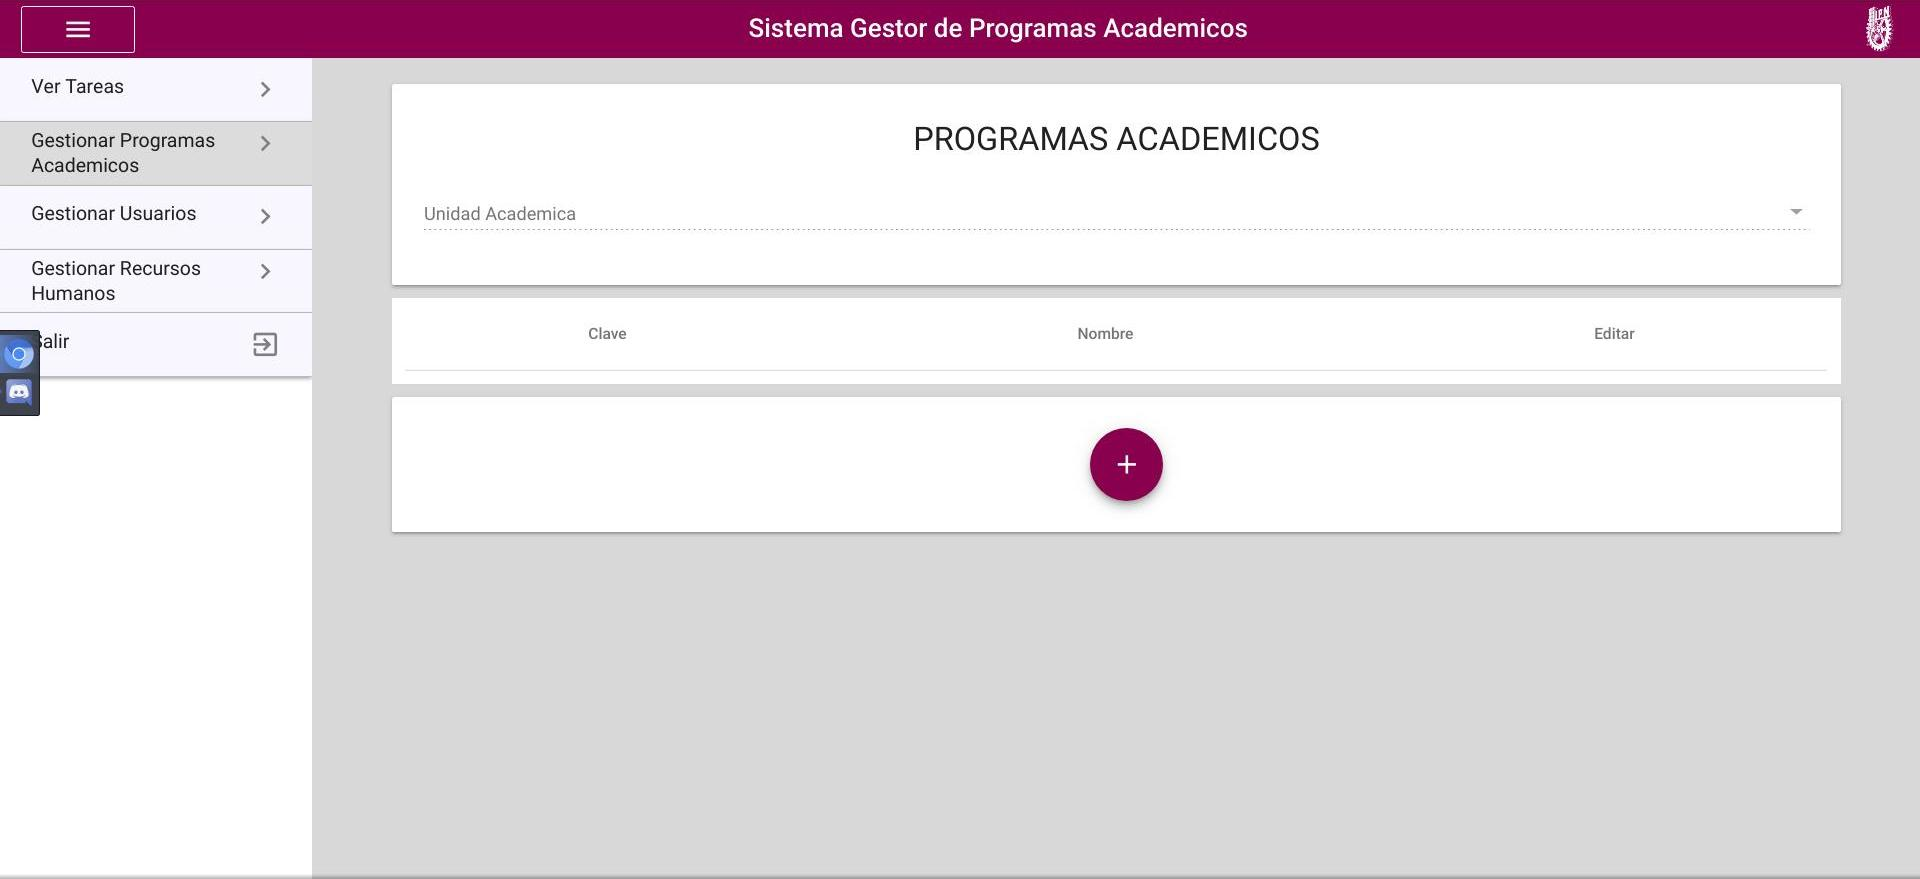
\includegraphics[width=0.7\linewidth]{images/SP3/ConsultarPA}}
        	\caption{Pantalla para Gestionar Programas Académicos}
        	\label{consultarpa}
        \end{figure}

        En donde aparecerá, de forma predeterminada, todos los Programas Académicos  registrados en el sistema al momento. Tendrá a su disposición 2 funciones:

	    \subsection{Editar Programa Académico}

        	Para ello, el usuario tendrá que dar clic en el botón con el icono de un lapiz amarillo que esta al lado del Programa Académico que desea modificar. Al hacer esto, el sistema redireccionará al usuario a la pantalla de \hyperlink{editarpa}{\textit{Editar Programa Académico}}.

        	\begin{figure}[!hbtp]
        		\centering
        		\hypertarget{editar}{
\includegraphics[width=0.7\linewidth]{images/SP3/BtnEditar}}
        		\caption{Botón Editar Programa Académico}
        		\label{editar}
        	\end{figure}

        \begin{figure}[!hbtp]
        	\centering
        	\hypertarget{editarpa}{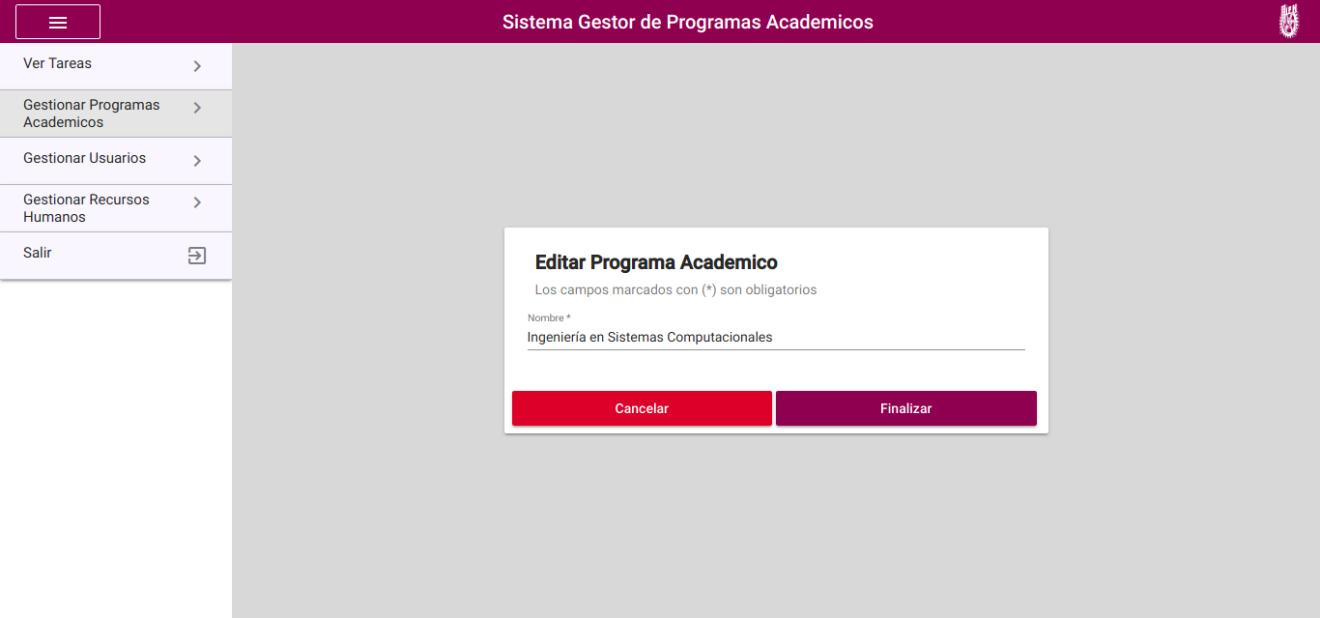
\includegraphics[width=0.7\linewidth]{images/SP3/EditarPA}}
        	\caption{Pantalla para la edición de Programas Académicos}
        	\label{editarpa}
        \end{figure}

        En donde se cargaran los datos del Programa Académico seleccionado en la pantalla de \hyperlink{consultarpa}{\textit{Consultar Programas Académicos}} y llenará el formulario.\\

        A continuación, el usuario puede modificar todos los campos del Programa Académico:
        \begin{figure}[!hbtp]
        	\centering
        	\hypertarget{modif}{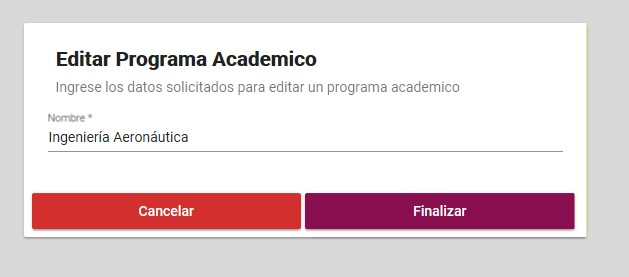
\includegraphics[width=0.7\linewidth]{images/SP3/Editado}}
        	\caption{Datos del Programa Académico modificados}
        	\label{modif}
        \end{figure}

        Si el usuario da clic en el botón ''Cancelar'' sin haber concluido la edición del Programa Académico:

        \begin{figure}[!hbtp]
        	\centering
        	\hypertarget{cancel2}{
\includegraphics[width=0.7\linewidth]{images/SP3/BtnCancelar}}
        	\caption{Botón ''Cancelar''}
        	\label{cancel2}
        \end{figure}

        El sistema mostrará el siguiente mensaje:
        %Imagen MSG29
        \begin{figure}[!hbtp]
            \centering
            \hypertarget{confirmar}{
\includegraphics[width=0.7\linewidth]{images/SP3/Confirmacion}}
            \caption{Confirmación}
            \label{confirmar}
        \end{figure}

        Para confirmar, el usuario debe dar clic en el botón ''Sí'', y el Programa Académico no será modificado.\\

        Para cancelar, el usuario debe dar clic en botón ''No'', el mensaje se cerrará y continuaremos en el formulario. Aqui el usuario puede terminar la edición del Programa Académico.\\

        Una vez verificados los datos, deberá de dar clic en el botón ''Finalizar''.
        \begin{figure}[!hbtp]
        	\centering
        	\hypertarget{btnfin}{
\includegraphics[width=0.7\linewidth]{images/SP3/BtnFinalizar}}
        	\caption{Botón ''Finalizar''}
        	\label{btnfin}
        \end{figure}

        Si no hubieron errores, el sistema muestra el siguiente mensaje:

        \begin{figure}[!hbtp]
            \centering
            \hypertarget{cambio}{
\includegraphics[width=0.7\linewidth]{images/SP3/Cambio}}
            \caption{Cambio exitoso.}
            \label{cambio}
        \end{figure}

        Al dar clic en en botón ''Aceptar'', el sistema redireccionará al usuario a la pantalla de \hyperlink{consultarpa}{\textit{Gestionar Programas Académicos}}, en donde podrá ver las modificaciones del Programa Académico.\\

        \subsubsection{Posibles errores}

            \begin{itemize}
            	\item Campos vacíos al momento de modificar el Programa Académico

                	Si el usuario dejo en blanco algún campo del formulario, el sistema mostrará el siguiente mensaje:

                    \begin{figure}[!hbtp]
                    \centering
                    \hypertarget{vacio}{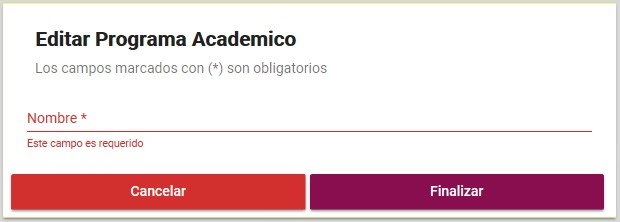
\includegraphics[width=0.7\linewidth]{images/SP3/Vacio}}
                    \caption{Campo Vacío}
                    \label{vacio}
                    \end{figure}

            	\item Los campos ingresados no son válidos

                	Si al momento de ingresar los datos aparece el siguiente mensaje:

                     \begin{figure}[!hbtp]
                    \centering
                    \hypertarget{invalido}{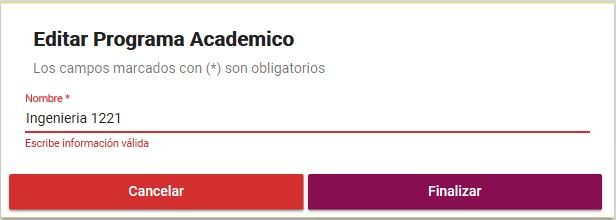
\includegraphics[width=0.7\linewidth]{images/SP3/Invalida}}
                    \caption{Campo Invalido}
                    \label{invalido}
                    \end{figure}


                	Significa que la composición de los datos ingresados en el formulario no es la correcta. Tenga en cuenta lo siguiente:

                	\begin{itemize}
                		\item El nombre se compone de únicamente de letras y espacios.

                        \item El nombre tiene una longitud máxima de 150 carácteres.
                	\end{itemize}

                \item El nombre del Programa Académico ya está registrado.
                    Si al momento de Finalizar la Edición muestra este mensaje.

                     \begin{figure}[!hbtp]
                    \centering
                    \hypertarget{vacio}{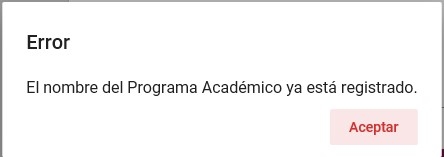
\includegraphics[width=0.7\linewidth]{images/SP3/Yareg}}
                    \caption{Campo Vacío}
                    \label{vacio}
                    \end{figure}

                    Significa que el Programa Académico ya ha sido registrado previamente dentro de la Unidad Académica.



            \end{itemize}
        \subsection{Registrar Programa Académico}

            Para ello, el usuario tendrá que dar clic en el botón ''+'' en la parte inferior de la pantalla.

            \begin{figure}[!hbtp]
                \centering
                \hypertarget{add}{
\includegraphics[width=0.7\linewidth]{images/SP3/BtnAgregar}}
                \caption{Botón Agregar Programa Académico}
                \label{add}
            \end{figure}

            Al hacerlo, el sistema redireccionará al usuario a la pantalla de \hyperlink{registrarpa}{\textit{Registrar Programa Académico}}.

        \begin{figure}[!hbtp]
            \centering
            \hypertarget{registrarpa}{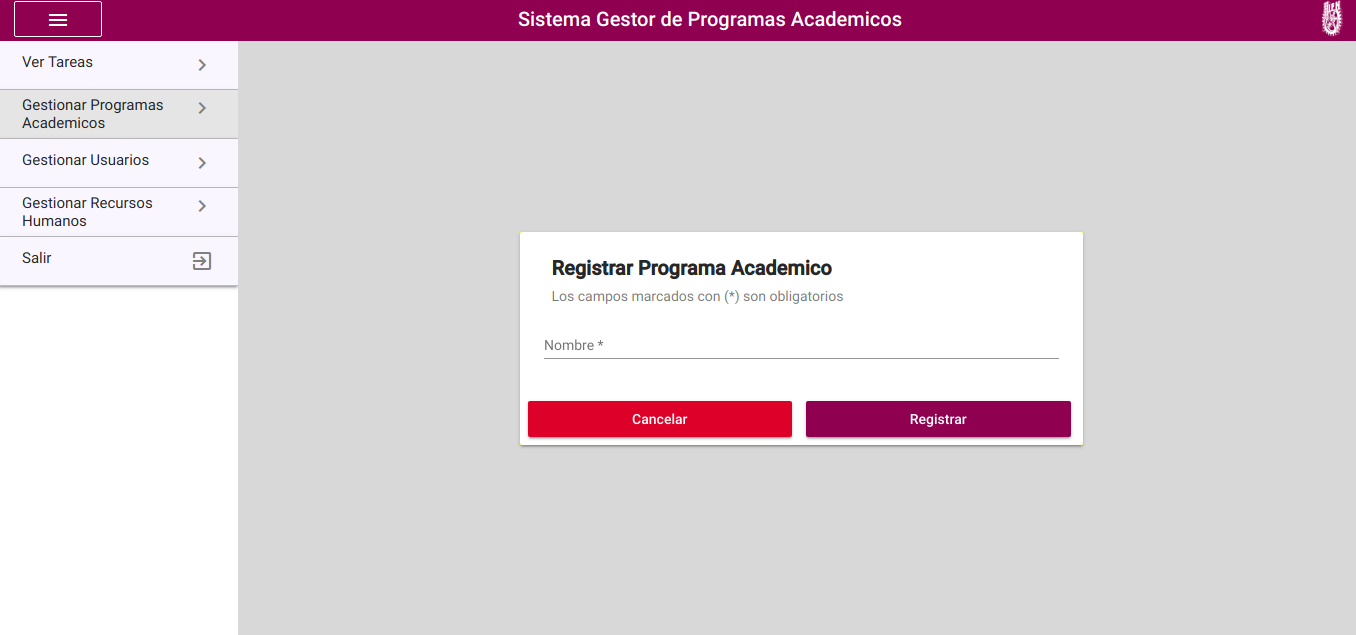
\includegraphics[width=0.7\linewidth]{images/SP3/RegistrarPA}}
            \caption{Pantalla para registrar Programas Académicos}
            \label{registrarpa}
        \end{figure}

        En donde tendrá que ingresar los campos del nuevo Programa Académico en el formulario. Un ejemplo del llenado sería el siguiente:

        \begin{figure}[!hbtp]
            \centering
            \hypertarget{ejreg}{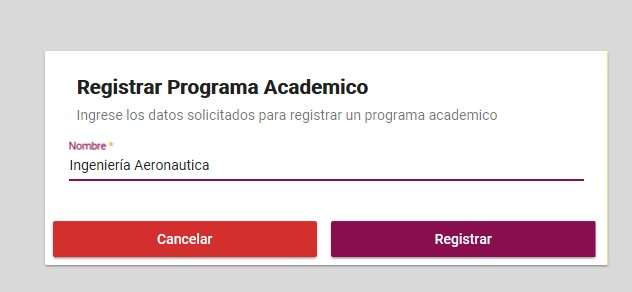
\includegraphics[width=0.7\linewidth]{images/SP3/Llenado}}
            \caption{Ejemplo de llenado para agregar un nuevo Programa Académico}
            \label{ejreg}
        \end{figure}

        Si el usuario da clic en el botón ''Cancelar'' sin haber concluido el registro del Programa Académico:

        \begin{figure}[!hbtp]
            \centering
            \hypertarget{cancel1}{
\includegraphics[width=0.7\linewidth]{images/SP3/BtnCancelar}}
            \caption{Botón ''Cancelar''}
            \label{cancel1}
        \end{figure}

         El sistema mostrará el siguiente mensaje:

        \begin{figure}[!hbtp]
            \centering
            \hypertarget{confirmar}{
\includegraphics[width=0.7\linewidth]{images/SP3/Confirmacion}}
            \caption{Confirmación}
            \label{confirmar}
        \end{figure}

        Para confirmar, el usuario debe dar clic en el botón ''Sí'', y el Programa Académico no será registrado.\\

        Para cancelar, el usuario debe dar clic en botón ''No'', el mensaje se cerrará y continuaremos en el formulario. Aqui el usuario puede terminar el registro.\\

        A continuación, una vez verificados los datos, deberá de dar clic en el botón ''Registrar''.
        \begin{figure}[!hbtp]
            \centering
            \hypertarget{btnreg}{
\includegraphics[width=0.7\linewidth]{images/SP3/BtnRegistrar}}
            \caption{Botón ''Registrar''}
            \label{btnreg}
        \end{figure}

        Si no hubieron errores, el sistema muestra el siguiente mensaje:

        \begin{figure}[!hbtp]
            \centering
            \hypertarget{exito}{
\includegraphics[width=0.7\linewidth]{images/SP3/Exitoso}}
            \caption{Registo exitoso.}
            \label{exito}
        \end{figure}

        Al dar clic en en botón ''Aceptar'', el sistema redireccionará al usuario a la pantalla de \hyperlink{consultarpa}{\textit{Gestionar Programas Académicos}}, en donde podrá ver el nuevo Programa Académico agregado.\\


        \subsubsection{Posibles errores}

            \begin{itemize}
                \item Campos vacíos al momento de modificar el Programa Académico

                    Si el usuario dejo en blanco algún campo del formulario, el sistema mostrará el siguiente mensaje:

                    \begin{figure}[!hbtp]
                    \centering
                    \hypertarget{vacio}{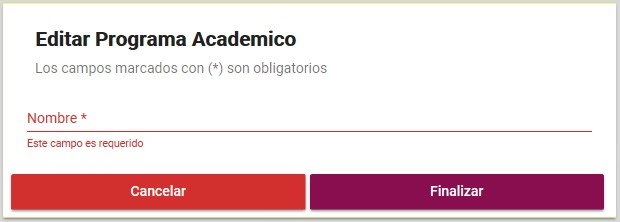
\includegraphics[width=0.7\linewidth]{images/SP3/Vacio}}
                    \caption{Campo Vacío}
                    \label{vacio}
                    \end{figure}

                \item Los campos ingresados no son válidos

                    Si al momento de ingresar los datos aparece el siguiente mensaje:

                     \begin{figure}[!hbtp]
                    \centering
                    \hypertarget{invalido}{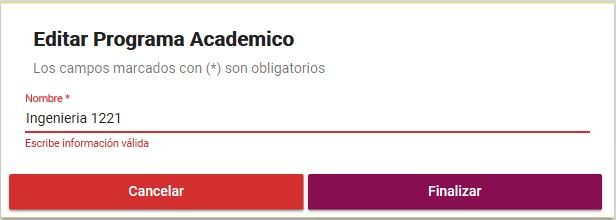
\includegraphics[width=0.7\linewidth]{images/SP3/Invalida}}
                    \caption{Campo Invalido}
                    \label{invalido}
                    \end{figure}


                    Significa que la composición de los datos ingresados en el formulario no es la correcta. Tenga en cuenta lo siguiente:

                    \begin{itemize}
                        \item El nombre se compone de únicamente de letras y espacios.

                        \item El nombre tiene una longitud máxima de 150 carácteres.
                    \end{itemize}

                \item El nombre del Programa Académico ya está registrado.
                    Si al momento de Finalizar la Edición muestra este mensaje.

                     \begin{figure}[!hbtp]
                    \centering
                    \hypertarget{vacio}{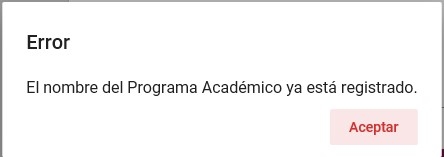
\includegraphics[width=0.7\linewidth]{images/SP3/Yareg}}
                    \caption{Campo Vacío}
                    \label{vacio}
                    \end{figure}

                    Significa que el Programa Académico ya ha sido registrado previamente dentro de la Unidad Académica.
            \end{itemize}
